\section{Experimental Work \& Results}
\subsection{Test Setup}
\begin{frame}
	\frametitle{Test Description}
	\begin{alertblock}{Hypothesis}
		\textit{``The networks that we use every day, have the necessary characteristics to
		generate the Bufferbloat phenomenon whether under low loads and if does exists, the how
	serious are the effects ?''}
	\end{alertblock}
\end{frame}
\begin{frame}
	\frametitle{Test Description}
	\begin{block}{Test Context}
		\begin{enumerate}
			\item Twice on the same day in one network to determine if does exist a considerable variance in latency for different times in a day.
			\item Select different public and private networks with different ``speeds''.
			\item Use the Ethernet cable in order to compare the results with those previo1usly obtained using Wireless.
		\end{enumerate}
	\end{block}
\end{frame}

\begin{frame}
	\begin{block}{Hardware}
		\begin{itemize}
			\item Physical Machine (Host Windows 7 OS)
			\item Virtual Machine (Kali Linux) 
			\item USB Wireless adapter (Zydas) + 8dbi antenna 
			\item Iperf Server / VPS\@Digital Ocean (NY DC)
		\end{itemize}
	\end{block}

	\begin{block}{Tools/Software}
		\begin{enumerate}[I]
			\item Speedtest.net $\rightarrow$ Base 
			\item Netalyzer $\rightarrow$ Characterization
			\item Iperf $\rightarrow$ Full Utilization
			\item Page Benchmark $\rightarrow$ User Experience
			\item Smokeping $\rightarrow$ Multiple Objectives
		\end{enumerate}
	\end{block}
\end{frame}

\subsection{Results}
\begin{frame}
	\frametitle{Speedtest.net}
	\begin{figure}[h!]
		\centering
		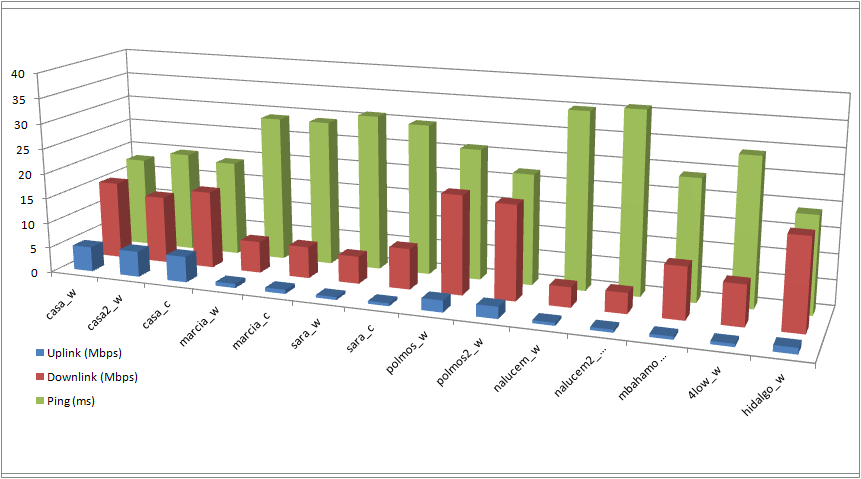
\includegraphics[scale=.45]{img/speed_graph}
		\caption{Speeds and Ping}
	\end{figure}
\end{frame}
\begin{frame}
	\frametitle{Results}
	\begin{block}{}
		\begin{itemize}
			\item The $\sim12ms$ ping were also not obtained, but the values are still within the acceptable range around the $\sim26ms$.
			\item The variation of the ratio between the measured and the bandwidth contracted is of 80\%, which is only 6\% less than spected.
		\end{itemize}
	\end{block}
\end{frame}


\begin{frame}
	\frametitle{Page Benchmark}
	\begin{figure}[h!]
		\centering
		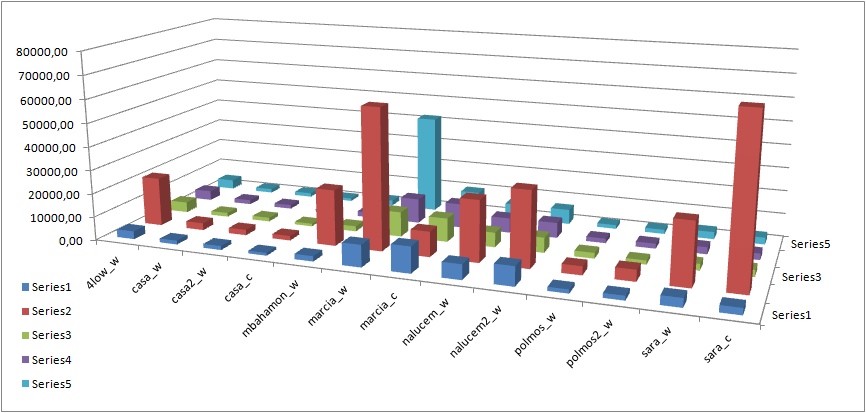
\includegraphics[scale=.45]{img/measures_page}
		\caption{Total Load Means in ms}
	\end{figure}
\end{frame}
\begin{frame}
	\frametitle{Results Overall}
	\begin{block}{}
		\begin{itemize}
			\item The average load for a problematic networks was over 9 (max 23) seconds. Normal load is between 1-7 (2) seconds. 
			\item The variation from minimun to maximum load was around 6 to 20 times.
		\end{itemize}
	\end{block}
\end{frame}

\begin{frame}
	\frametitle{Smokeping}
	\begin{figure} 
		\begin{subfigure}{\textwidth} 
			\centering 
			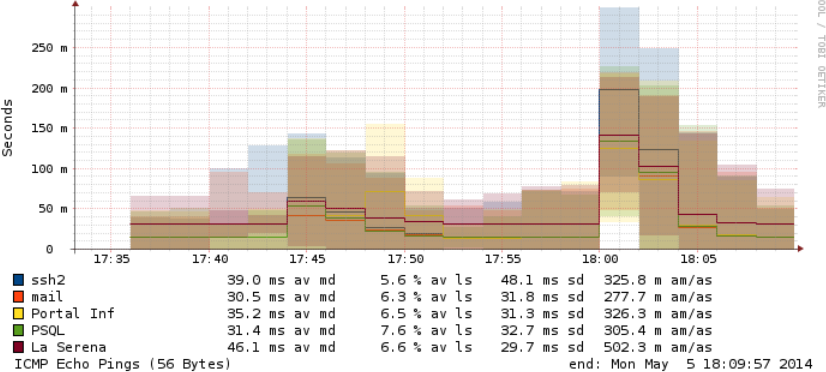
\includegraphics[width=0.6\textwidth]{img/smoke_nat_good} 
			\caption[Smokeping: Ping test to National servers with good performance]{Good performance Network} 
		\end{subfigure}% 
		\\ 
		\begin{subfigure}{\textwidth} 
			\centering 
			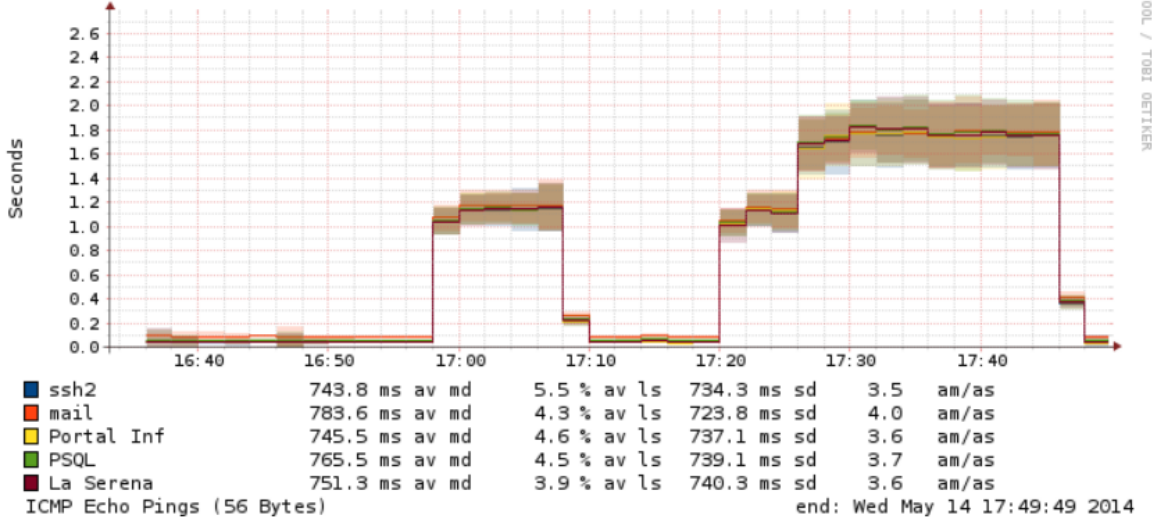
\includegraphics[width=0.6\textwidth]{img/smoke_nat_bad} 
			\caption[Smokeping: Ping test to National servers with bad performance]{Bad performance Network} 
		\end{subfigure} 
		\caption{Ping test to National servers} 
	\end{figure} 
\end{frame}


\begin{frame}
	\frametitle{Smokeping}
	\begin{figure}[h!]
		\centering 
		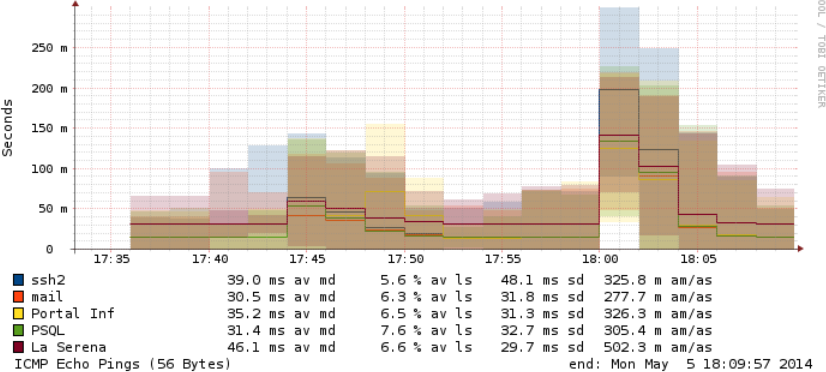
\includegraphics[scale=.35]{img/smoke_nat_good} 
		\caption[Smokeping: Ping test to National servers with good performance]{Good performance Network} 
	\end{figure}% 
\end{frame}
\begin{frame}
	\frametitle{Smokeping}
	\begin{figure}[h!]
			\centering 
			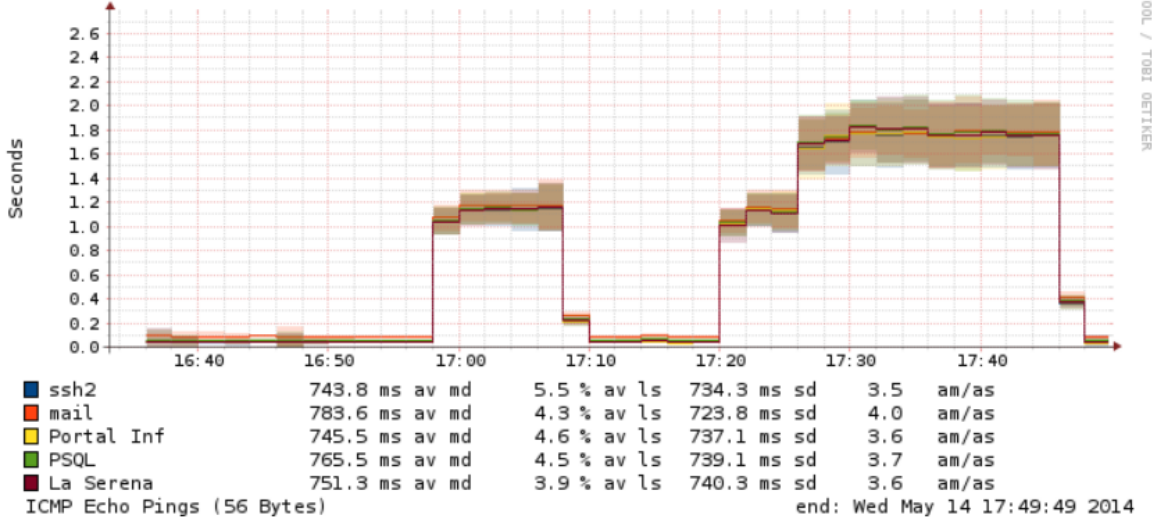
\includegraphics[scale=.35]{img/smoke_nat_bad} 
			\caption[Smokeping: Ping test to National servers with bad performance]{Bad performance Network} 
	\end{figure} 
\end{frame}


\begin{frame}
	\frametitle{Smokeping}
	\begin{figure} 
		\begin{subfigure}{\textwidth} 
			\centering 
			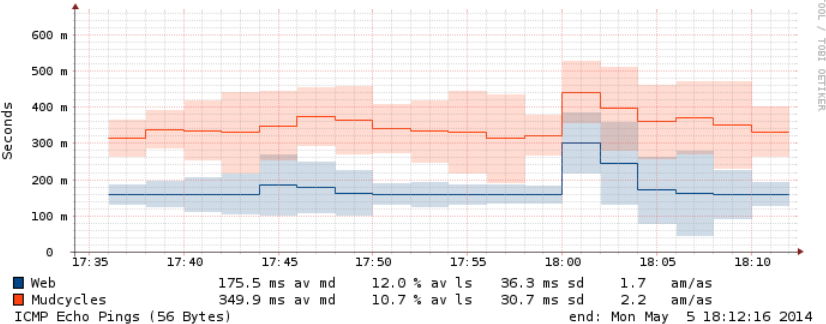
\includegraphics[width=0.6\textwidth]{img/smoke_int_good}
			\caption[Smokeping: Ping test to International Servers with good performance]{Good performance network}
		\end{subfigure}% 
		\\ 
		\begin{subfigure}{\textwidth} 
			\centering 
			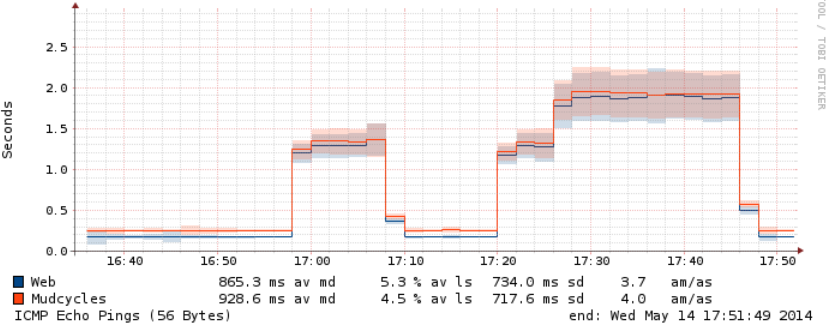
\includegraphics[width=0.6\textwidth]{img/smoke_int_bad}
			\caption[Smokeping: Ping test to International servers with bad performance]{Bad performance network}
		\end{subfigure}
		\caption[Smokeping: Ping test to International servers]{Ping test to International servers}
	\end{figure} 
\end{frame}


\begin{frame}
	\frametitle{Smokeping}
	\begin{figure}[h!]
		\centering 
			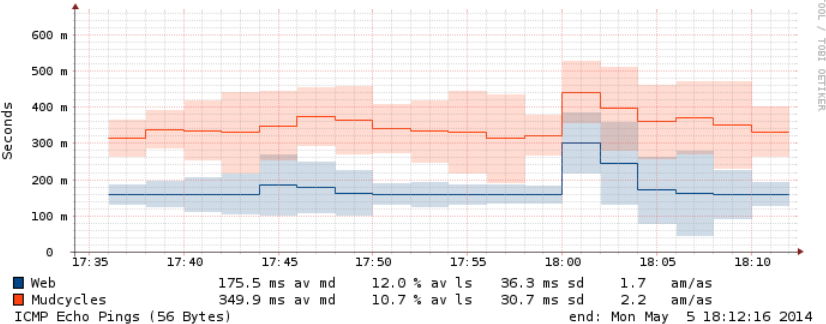
\includegraphics[scale=0.35]{img/smoke_int_good}
			\caption[Smokeping: Ping test to International Servers with good performance]{Good performance network}
	\end{figure}% 
\end{frame}
\begin{frame}
	\frametitle{Smokeping}
	\begin{figure}[h!] 
		\centering 
		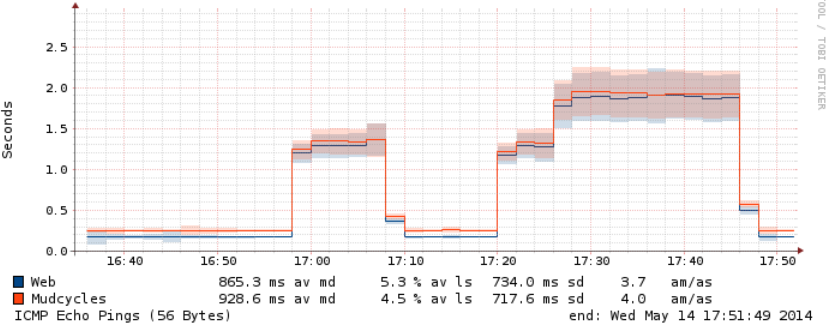
\includegraphics[scale=.35]{img/smoke_int_bad}
		\caption[Smokeping: Ping test to International servers with bad performance]{Bad performance network}
	\end{figure}
\end{frame}



\begin{frame}
	\frametitle{Smokeping}
	\begin{figure} 
		\begin{subfigure}{\textwidth} 
			\centering 
			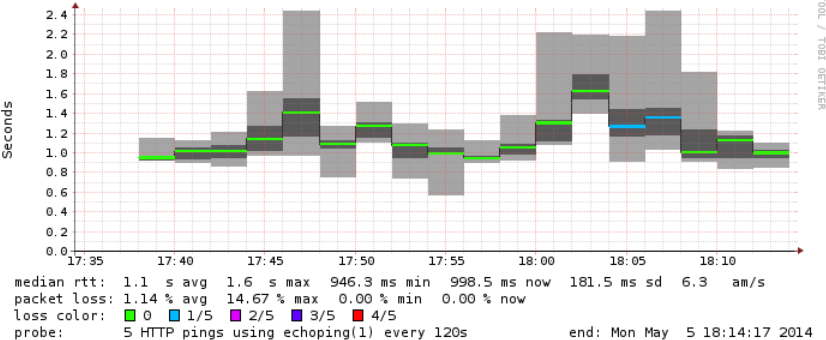
\includegraphics[width=0.6\textwidth]{img/smoke_inf_good}
			\caption[Smokeping: Web requests with good performance]{Good performance network}
		\end{subfigure}% 
		\\ 
		\begin{subfigure}{\textwidth} 
			\centering 
			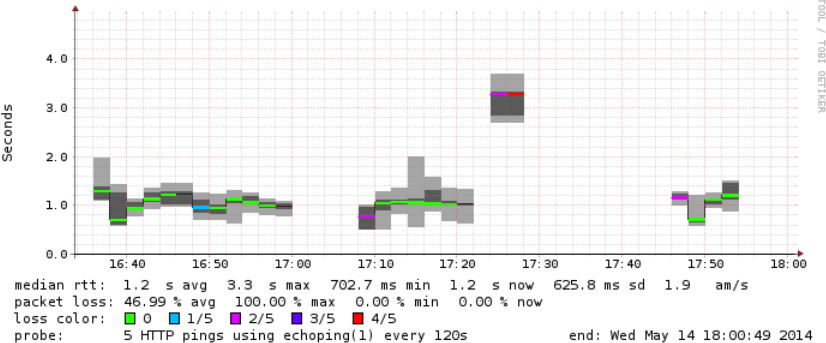
\includegraphics[width=0.6\textwidth]{img/smoke_inf_bad}
			\caption[Smokeping: Web requests with bad performance]{Bad performance network}
		\end{subfigure}
		\caption[Smokeping: Web requests to National servers]{Web requests to National servers}

	\end{figure} 
\end{frame}


\begin{frame}
	\frametitle{Smokeping}
	\begin{figure}[h!]
		\centering 
			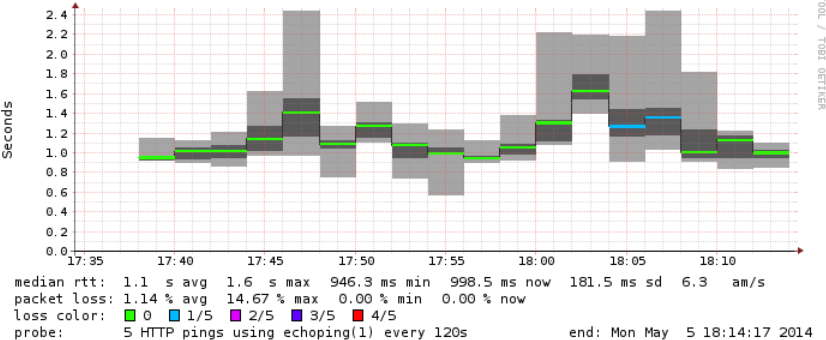
\includegraphics[scale=0.35]{img/smoke_inf_good}
			\caption[Smokeping: Web requests with good performance]{Good performance network}
	\end{figure}% 
\end{frame}
\begin{frame}
	\frametitle{Smokeping}
	\begin{figure}[h!]
			\centering 
			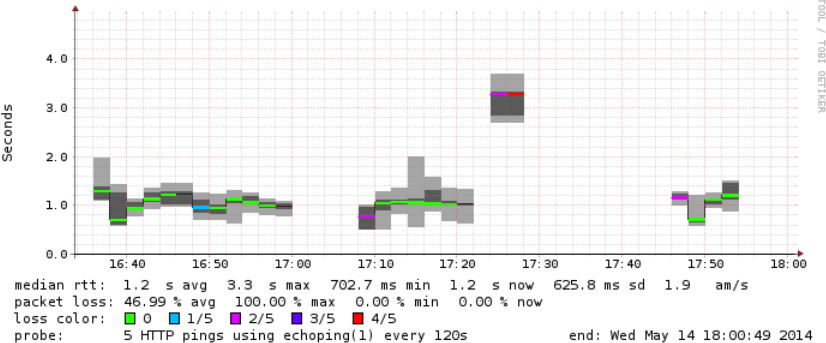
\includegraphics[scale=0.35]{img/smoke_inf_bad}
			\caption[Smokeping: Web requests with bad performance]{Bad performance network}
	\end{figure} 
\end{frame}
\begin{frame}
	\frametitle{Results Overall}
	\begin{block}{}
		\begin{itemize}
			\item The range for latency in a problematic network can be from 250ms to about 2 seconds.
			\item Lost related to problematic network can be over 70\% with 3 seconds to load and can reach to fully lost of communication.
		\end{itemize}
	\end{block}
\end{frame}

